Textured and colored pavements refers to the use of varied pavement materials to alter the color or texture of a street surface. This practice can be used as a traffic calming measure or as a way to distinguish special areas of the street.

Changes in pavement texture from normal concrete or asphalt surfaces can cause a change in audible road noise inside the car body. This effect can be utilized to alert drivers to slow down or take notice of potential hazards. Textured or colored pavements can also be used to visually distinguish special areas of the street, such as crosswalks or bike lanes, to make drivers more aware of their location \cite{TP1}.

Altered pavement textures and colors have been found to cause reductions in vehicle speed, though there is limited data available to quantify this \cite{TP3}. This practice can be used in combination with other practices to produce a traffic calming effect, such as raised crosswalks, speed tables, or raised intersections. 

\subsubsection{Materials}

\paragraph{Cobblestones} Cobblestone roads are paved with quarried stone with rounded tops. The advantages of this material are that it will create a significant audible disturbance to drivers and can provide a unique aesthetic appeal; however, cyclists and wheelchair users might find this pavement difficult to navigate. Additionally, the unevenness of the pavement makes it more difficult to remove snow and ice \cite{TP6}.

\begin{figure}[h]
\centering
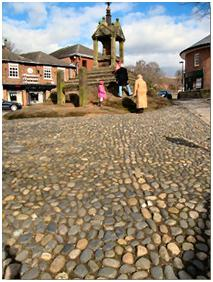
\includegraphics[width=0.5\textwidth]{TPA.jpg}
\caption[Cobblestone street in Lymm Cross, Cheshire, England]{Cobblestone street in Lymm Cross, Cheshire, England}\label{fig:TPA}
\end{figure}

\paragraph{Setts and Bricks} Setts are quarried stone blocks that are flat-topped (in contrast with round-topped cobblestones). They are typically arranged in a uniform matter, as pictured in \figref{TPBC}. Bricks are used and placed in a similar nature, but come from a different source material.  The road texture of sett-paved roads can vary depending on the evenness of the selected setts \cite{TP4}.

\begin{figure}[h]
\centering
	\begin{subfigure}[t]{0.4\textwidth}
		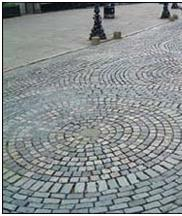
\includegraphics[width=\textwidth]{TPB.jpg}
	\end{subfigure}
	\begin{subfigure}[t]{0.4\textwidth}
		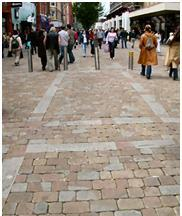
\includegraphics[width=\textwidth]{TPC.jpg}
	\end{subfigure}
\caption{Streets paved with setts}\label{fig:TPBC}
\end{figure}



\begin{figure}[h]
\centering
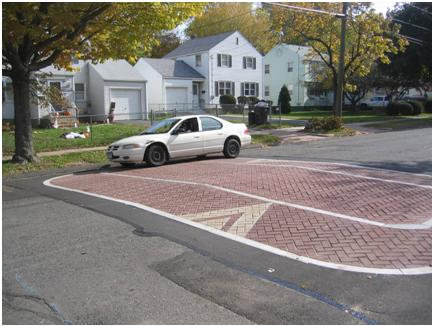
\includegraphics[width=0.5\textwidth]{TPD.jpg}
\caption[Speed hump utilizing brick paving]{Speed hump utilizing brick paving}\label{fig:TPD}
\end{figure}

\paragraph{Concrete Blocks} Concrete blocks are pre-cast, individual blocks of concrete that are placed similarly to bricks or setts. An advantage of using concrete blocks is that they can be shaped and colored in different ways to create a desired appearance. For example, concrete blocks can be made to look like setts and bricks by casting them in a certain size and applying the proper coloring. An additional advantage of concrete blocks is their reduced cost \cite{TP5}.

\begin{figure}[h]
\centering
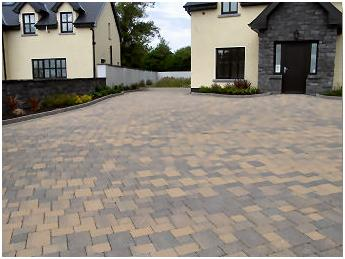
\includegraphics[width=0.5\textwidth]{TPE.jpg}
\caption[Concrete block paving]{Concrete block paving}\label{fig:TPE}
\end{figure}

\paragraph{Colored Pavement}Pavement can be colored through the use of pavement striping paint, as similarly used to make normal pavement markings. While textured pavements generally are made up of more earthen tones, bright colors can be used to create a very noticeable visual effect, as demonstrated by the green bike lanes in \figref{TPF}.

\begin{figure}[h]
\centering
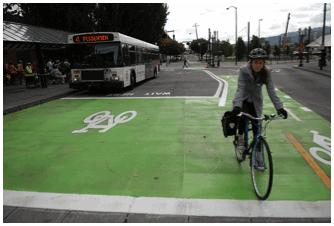
\includegraphics[width=0.5\textwidth]{TPF.jpg}
\caption[Green-colored bike lanes in Portland]{Green-colored bike lanes in Portland}\label{fig:TPF}
\end{figure}


\begin{figure}[h]
\centering
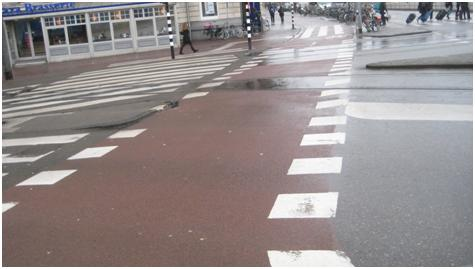
\includegraphics[width=0.5\textwidth]{TPG.jpg}
\caption[Brown coloring used to distinguish a bike path crossing in the Netherlands]{Brown coloring used to distinguish a bike path crossing in the Netherlands}\label{fig:TPG}
\end{figure}

\subsubsection{Cost}

The cost of utilizing textured or color pavements is dependent on a) the material used and b) the total area of the pavement. The Victoria Transport Policy Institute estimates a cost range of $5-$16 per square foot \cite{TP3}. A crosswalk 10 feet in width crossing a four-lane road, for example, would have a total material cost ranging from $2400 to $7680.
